\phantomsection
\subsection*{\normalsize Longstaff--Schwartz Regression Method for American Puts}
\label{app:mc_lsm_option}

\paragraph{Contract and risk-neutral simulation.}
The option is an American put with payoff
\[
    h(S)=\max(K-S,0).
\]
Under the risk-neutral measure,
\[
    dS_t=rS_t\,dt+\sigma S_t\,dW_t.
\]
As in the paper's Table~1 experiment, the stock pays no dividends and
\(r,\sigma\) are constant.
On an exercise grid with \(N=50T\) intervals and
\(\Delta t=T/N=1/50\) years, stock paths are generated by the exact
geometric-Brownian-motion transition
\[
    S_{i+1}
    =S_i\exp\!\left[
        \left(r-\frac{\sigma^2}{2}\right)\Delta t
        +\sigma\sqrt{\Delta t}\,Z_{i+1}
    \right],
    \qquad Z_{i+1}\sim\mathcal{N}(0,1).
\]
The contract settings follow the American-put experiment in
Longstaff and Schwartz (2001), Table~1:
\[
    K=40,\qquad r=0.06,\qquad
    S_0\in\{36,38,40,42,44\},\qquad
    \sigma\in\{0.20,0.40\},\qquad T\in\{1,2\}.
\]
There are 50 exercise dates per year, hence 50 or 100 exercise intervals
for the one- or two-year contracts.

\paragraph{Continuation-value regression.}
At each date, the continuation value is approximated by least squares.
Following the notation and state variable in Longstaff and Schwartz,
we use the stock price itself \(X=S\), without dividing by the strike or
otherwise normalizing the state. The basis is a constant and the first
three weighted Laguerre functions:
\[
    \{1,L_0(X),L_1(X),L_2(X)\},\qquad
    L_0(X)=e^{-X/2},\quad
    L_1(X)=e^{-X/2}(1-X),\quad
    L_2(X)=e^{-X/2}\left(1-2X+\frac{X^2}{2}\right).
\]
The numerical least-squares solver equilibrates regressor columns internally
and transforms the fitted coefficients back; this improves numerical
stability without changing the state variable or the fitted basis.
The state is not strike-normalized.
The fitted continuation value is
\[
    \widehat C_i(S)
    =\max\!\left\{0,\,
      \boldsymbol{\phi}(S)^{\mathsf T}
      \widehat{\boldsymbol\beta}_i\right\}.
\]
The zero floor enforces the nonnegative value of an option when a fitted
polynomial is negative.

\paragraph{Related TVR recursion (mathematical context only).}
Tsitsiklis and Van Roy (2001), ``Regression Methods for Pricing Complex
American-Style Options,'' also approximate continuation values by regression.
For context, their backward recursion can be written
\[
    \widehat{\boldsymbol\theta}_i
    =\underset{\boldsymbol\theta}{\arg\min}
      \sum_{m=1}^{M}
      \left[
        e^{-r\Delta t}\widehat V_{i+1}(S_{i+1,m})
        -\boldsymbol{\phi}(S_{i,m})^{\mathsf T}\boldsymbol\theta
      \right]^2,
    \qquad
    \widehat V_i(S)
    =\max\!\left\{h(S),
      \boldsymbol{\phi}(S)^{\mathsf T}\widehat{\boldsymbol\theta}_i
      \right\}.
\]
This recursion is included only to acknowledge the related method; TVR is
not implemented and none of the numerical tables or figures below report
TVR results.

\paragraph{Longstaff--Schwartz algorithm.}
At maturity, each path receives its put payoff. Moving backward in time,
LSM considers paths that are in the money at date \(t_i\),
\(S_{i,m}<K\). Let \(Y_{i,m}\) be the cash flow from the future exercise
date currently selected for path \(m\), discounted back to \(t_i\). The
regression is
\[
    \widehat{\boldsymbol\beta}_i
    =
    \underset{\boldsymbol\beta}{\arg\min}
    \sum_{m:S_{i,m}<K}
    \left[
        Y_{i,m}
        -\boldsymbol{\phi}(S_{i,m})^{\mathsf T}\boldsymbol\beta
    \right]^2.
\]
The path is exercised when immediate exercise is more valuable than
estimated continuation:
\[
    \text{exercise at }t_i
    \quad\Longleftrightarrow\quad
    h(S_{i,m})>\widehat C_i(S_{i,m}).
\]
At time zero, all paths have the same known stock price, so no cross-sectional
regression is required. The initial exercise payoff is compared with the
sample mean of the fitted-policy cash flows discounted back to time zero.
The option estimate is the mean of the discounted realized payoffs from
following this fitted stopping rule. This is the in-sample valuation
protocol used for the paper-style table.

\paragraph{Plain Monte Carlo and antithetic variates.}
The paper-style run uses 100,000 paths with antithetic sampling: every
normal-shock sequence \((Z_1,\ldots,Z_N)\) is paired with
\((-Z_1,\ldots,-Z_N)\). Its standard error is computed from the 50,000
pair-average discounted payoffs. The plain-Monte-Carlo comparison uses
100,000 unpaired paths with the same contract settings and basis. If
\(X_m\) are the independent observations (single-path payoffs for plain
MC and pair averages for AV), then
\[
    \widehat V=\frac{1}{n}\sum_{m=1}^{n}X_m,\qquad
    \widehat{\operatorname{SE}}(\widehat V)
    =\frac{s_X}{\sqrt{n}},
\]
where \(s_X\) is the sample standard deviation. A nominal 95\% interval
is \(\widehat V\pm1.96\,\widehat{\operatorname{SE}}\).

\paragraph{CRR benchmark.}
For each contract, the reference is a 2,000-step Cox--Ross--Rubinstein
(CRR) tree with exercise opportunities aligned to the same 50-per-year
schedule. For tree time step \(\delta t=T/J\), \(J=2{,}000\),
\[
    u=e^{\sigma\sqrt{\delta t}},\qquad
    d=u^{-1},\qquad
    p=\frac{e^{r\delta t}-d}{u-d},\qquad
    S_{j,k}=S_0u^kd^{\,j-k}.
\]
Set \(V_{J,k}=h(S_{J,k})\). At each earlier node, compute
\[
    C_{j,k}
    =e^{-r\delta t}
      \left[pV_{j+1,k+1}+(1-p)V_{j+1,k}\right],
\]
then apply
\[
    V_{j,k}=
    \begin{cases}
        \max\{h(S_{j,k}),C_{j,k}\},
            & j\text{ is an allowed exercise date},\\
        C_{j,k},&\text{otherwise}.
    \end{cases}
\]
The resulting \(V_{0,0}\) is a Bermudan-tree benchmark on the Monte Carlo
exercise grid. It is not the finite-difference reference reported in the
original paper. The absolute pricing error in the tables is
\[
    \left|\widehat V_{\mathrm{LSM}}-V_{0,0}^{\mathrm{CRR}}\right|.
\]

\paragraph{How this experiment compares with Longstaff--Schwartz Table~1.}
The contract grid follows the paper's Table~1 settings:
\(K=40\), \(r=6\%\), the same five initial spots, two volatilities,
one- and two-year maturities, and 50 exercise opportunities per year.
The table below places the paper's published LSM estimate and reported
standard error beside our native C++ antithetic estimate and standard
error. It also shows the signed AV-minus-paper difference, our 2,000-step
Bermudan CRR reference, and the plain-MC baseline with its absolute CRR
error. The paper's finite-difference price is discussed as its original
benchmark but is not included in this simulation-to-simulation table.

These columns answer different comparison questions. The published LSM
column checks whether our estimates are in the range of the paper's
simulation result; the paper's finite-difference value is its original
numerical reference. Our CRR column is a separate, exercise-grid-matched
Bermudan benchmark used to measure errors consistently for this project.
It is not the paper's finite-difference value, so the two references must
not be treated as interchangeable. Each maturity's table places these
comparisons together: the AV-minus-paper column is signed, while the
plain-MC-versus-CRR column is an absolute error.

The native LSM now uses the unnormalized stock-price state \(X=S\) and
basis functions directly, following the paper's notation and the
direct-state interpretation requested for this benchmark. The reported
contract settings are matched, but this is not an exact reproduction of
the paper's random paths, implementation details, or reference
calculation. We use 100,000 total paths
and seed 42 for each native run; the AV run comprises 50,000 shock pairs
(100,000 paths). Plain MC is our added no-variance-reduction comparison.
The paper reports its own antithetic simulation result, not a plain-MC
estimate. It computes its finite-difference values using 40,000 time steps
per year and 1,000 stock-price steps; our CRR benchmark is a separate
2,000-step tree. In the paper, the table's reported American prices are
total option values; its early-exercise premium is the American value minus
the Black--Scholes European put value.
\paragraph{Observed comparison.}
For the direct, unnormalized stock-price basis, every one of our 20 AV
estimates is below the paper's published LSM estimate. The mean absolute
difference is about \(0.2974\), and none of the 20 differences is within
1.96 combined standard errors. At \(S_0=K=40\), \(\sigma=20\%\), and
\(T=1\), for example, our AV estimate is \(2.2567\), compared with the
paper's \(2.313\) and our CRR reference \(2.3140\). This is a material
discrepancy, not evidence that the paper's results have been reproduced.
It shows that, although we have now kept the stock variable unnormalized
as requested, this direct-state basis implementation does not match the
paper's numerical LSM results. The weighted functions
\(e^{-S/2}\{1,1-S,1-2S+S^2/2\}\) become very small over much of the
stock-price range in these examples, which can make the fitted exercise
policy ineffective. The CRR column makes this discrepancy visible; it is
a reference, not a calibration target. AV standard errors are computed
from independent pair averages and were lower than plain-MC standard
errors in all 20 cases, but lower variance does not correct this
approximation discrepancy.
% Generated by run_report.py from paper_table.csv.
% Published LSM values transcribed from Longstaff-Schwartz (2001), Table 1.
\begin{table}[!htbp]
    \centering\scriptsize
    \caption{Longstaff--Schwartz Table~1 comparison, \(T=1\) year(s).}
    \label{tab:lsm_paper_comparison_t1}
    \setlength{\tabcolsep}{3pt}
    \begin{tabular*}{\linewidth}{@{\extracolsep{\fill}}rr|rrrrrr}
        \toprule
        \(S_0\) & \(\sigma\) & \multicolumn{3}{c|}{Published comparison} & \multicolumn{3}{c}{Our estimates and CRR errors} \\
        \cmidrule(lr){3-5}\cmidrule(lr){6-8}
        & & Paper LSM (SE) & AV LSM (SE) & AV $-$ paper & CRR reference & Plain MC (SE) & \(|V_{\rm plain}-V_{\rm CRR}|\) \\
        \midrule
        36 & 20\% & 4.472 (0.010) & 4.4078 (0.0052) & -0.0642 & 4.4780 & 4.4112 (0.0076) & 0.0668 \\
        38 & 20\% & 3.244 (0.009) & 3.1838 (0.0046) & -0.0602 & 3.2504 & 3.1845 (0.0078) & 0.0659 \\
        40 & 20\% & 2.313 (0.009) & 2.2567 (0.0042) & -0.0563 & 2.3140 & 2.2533 (0.0073) & 0.0607 \\
        42 & 20\% & 1.617 (0.007) & 1.5687 (0.0045) & -0.0483 & 1.6173 & 1.5697 (0.0066) & 0.0476 \\
        44 & 20\% & 1.118 (0.007) & 1.0741 (0.0045) & -0.0439 & 1.1101 & 1.0754 (0.0057) & 0.0347 \\
        36 & 40\% & 7.091 (0.020) & 6.6077 (0.0098) & -0.4833 & 7.1014 & 6.6170 (0.0132) & 0.4843 \\
        38 & 40\% & 6.139 (0.019) & 5.6808 (0.0090) & -0.4582 & 6.1478 & 5.7115 (0.0134) & 0.4363 \\
        40 & 40\% & 5.308 (0.018) & 4.8931 (0.0078) & -0.4149 & 5.3116 & 4.9265 (0.0133) & 0.3851 \\
        42 & 40\% & 4.588 (0.017) & 4.2323 (0.0072) & -0.3557 & 4.5830 & 4.2376 (0.0129) & 0.3454 \\
        44 & 40\% & 3.957 (0.017) & 3.6388 (0.0072) & -0.3182 & 3.9483 & 3.6525 (0.0124) & 0.2958 \\
        \bottomrule
    \end{tabular*}
    \begin{minipage}{0.96\linewidth}\footnotesize
    AV $-$ paper is our antithetic estimate minus the published LSM estimate. Our CRR is a separate 2,000-step Bermudan reference, not the paper's finite-difference value.
    Plain MC is our added no-variance-reduction baseline; published prices and standard errors are rounded as in Table~1.
    \end{minipage}
\end{table}

\begin{table}[!htbp]
    \centering\scriptsize
    \caption{Longstaff--Schwartz Table~1 comparison, \(T=2\) year(s).}
    \label{tab:lsm_paper_comparison_t2}
    \setlength{\tabcolsep}{3pt}
    \begin{tabular*}{\linewidth}{@{\extracolsep{\fill}}rr|rrrrrr}
        \toprule
        \(S_0\) & \(\sigma\) & \multicolumn{3}{c|}{Published comparison} & \multicolumn{3}{c}{Our estimates and CRR errors} \\
        \cmidrule(lr){3-5}\cmidrule(lr){6-8}
        & & Paper LSM (SE) & AV LSM (SE) & AV $-$ paper & CRR reference & Plain MC (SE) & \(|V_{\rm plain}-V_{\rm CRR}|\) \\
        \midrule
        36 & 20\% & 4.821 (0.012) & 4.7157 (0.0061) & -0.1053 & 4.8405 & 4.7168 (0.0086) & 0.1237 \\
        38 & 20\% & 3.735 (0.011) & 3.6170 (0.0057) & -0.1180 & 3.7448 & 3.6264 (0.0087) & 0.1184 \\
        40 & 20\% & 2.879 (0.010) & 2.7697 (0.0051) & -0.1093 & 2.8845 & 2.7603 (0.0084) & 0.1242 \\
        42 & 20\% & 2.206 (0.010) & 2.1094 (0.0051) & -0.0966 & 2.2125 & 2.1142 (0.0079) & 0.0984 \\
        44 & 20\% & 1.675 (0.009) & 1.6115 (0.0053) & -0.0635 & 1.6902 & 1.6150 (0.0072) & 0.0752 \\
        36 & 40\% & 8.488 (0.024) & 7.7343 (0.0118) & -0.7537 & 8.5072 & 7.7876 (0.0150) & 0.7196 \\
        38 & 40\% & 7.669 (0.022) & 6.9638 (0.0112) & -0.7052 & 7.6679 & 6.9931 (0.0152) & 0.6748 \\
        40 & 40\% & 6.921 (0.022) & 6.2923 (0.0102) & -0.6287 & 6.9167 & 6.2917 (0.0153) & 0.6250 \\
        42 & 40\% & 6.243 (0.021) & 5.6731 (0.0093) & -0.5699 & 6.2443 & 5.6703 (0.0152) & 0.5740 \\
        44 & 40\% & 5.622 (0.021) & 5.1272 (0.0087) & -0.4948 & 5.6418 & 5.1269 (0.0150) & 0.5149 \\
        \bottomrule
    \end{tabular*}
    \begin{minipage}{0.96\linewidth}\footnotesize
    AV $-$ paper is our antithetic estimate minus the published LSM estimate. Our CRR is a separate 2,000-step Bermudan reference, not the paper's finite-difference value.
    Plain MC is our added no-variance-reduction baseline; published prices and standard errors are rounded as in Table~1.
    \end{minipage}
\end{table}


\paragraph{Convergence experiment.}
To illustrate how uncertainty changes with sample size, we use the
at-the-money case \(S_0=K=40\), separately at \(\sigma=20\%\) and
\(\sigma=40\%\), with \(T=1\). Each combination of path count and sampling
scheme is repeated with 30 independent seeds, \(42,\ldots,71\), at
\[
    M\in\{5{,}000,\;10{,}000,\;25{,}000,\;50{,}000,\;100{,}000\}.
\]
For each path count and scheme, the plotted center is the mean of the 30
price estimates. The interval is a 95\% Student-\(t\) interval across
replications:
\[
    \overline V
    \pm t_{0.975,29}\frac{s_{\mathrm{rep}}}{\sqrt{30}},
    \qquad t_{0.975,29}=2.0452,
\]
where \(s_{\mathrm{rep}}\) is the standard deviation of the 30 run-level
estimates. Unlike a single-run path standard error, this interval also
reflects observed run-to-run variation in fitted policies.

\begin{figure}[htbp]
    \centering
    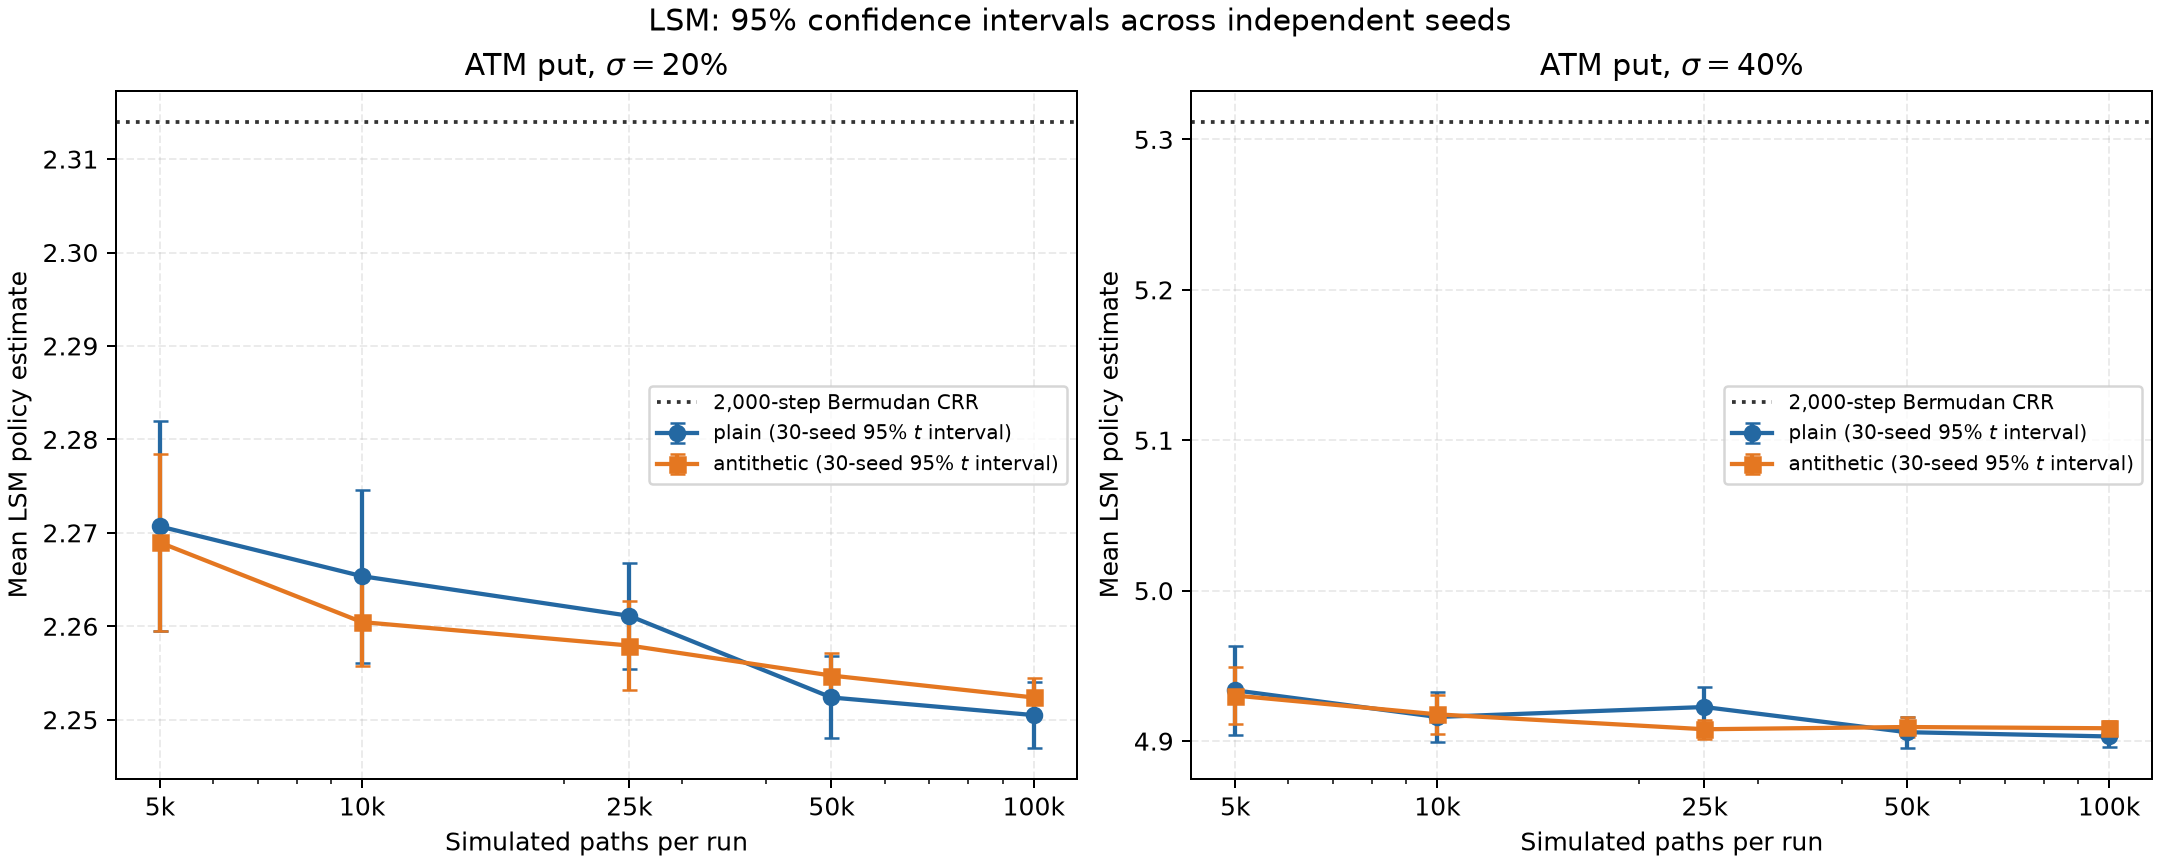
\includegraphics[width=\linewidth]{lsm_confidence_intervals.png}
    \caption{LSM mean estimates and 95\% Student-\(t\) intervals across 30
    independent seeds, by path count. Panels show the two volatility cases.
    The dotted line is the matching 2,000-step Bermudan CRR benchmark.}
    \label{fig:lsm_confidence_intervals}
\end{figure}

Across all ten volatility/path-count combinations, the antithetic runs
have lower seed-to-seed standard deviation than plain MC; the reduction
ranges from \(15.2\%\) to \(52.6\%\), averaging \(33.9\%\). The mean
single-run standard error is also lower for AV in every combination,
averaging a \(41.9\%\) reduction. This is evidence of reduced sampling
variation, not of more accurate prices: plain and AV means can differ, and
both remain below the CRR reference in this direct-\(S\) basis experiment.
The confidence intervals may still overlap. A narrower interval does not
remove approximation error or replace a separate out-of-sample policy
evaluation, since the regression policy is fitted and valued on the same
paths in each run.

\paragraph{Exercise boundary and sample paths.}
For each fitted date-\(t_i\) regression, the immediate and continuation
values are evaluated over 1,001 equally spaced stock prices from \(0.01K\)
to \(K\). The plotted exercise boundary is the largest grid price at
which immediate exercise is preferred:
\[
    \widehat B_i
    =
    \max\left\{S\in[0.01K,K]:
        h(S)>\widehat C_i(S)\right\}.
\]
For a put, prices below this estimated boundary are classified as the
exercise region. The boundary is set to \(K\) at maturity. The figure
overlays the fitted boundary and a sample of simulated paths for the
at-the-money case with \(T=1\), \(\sigma=20\%\), and 100,000 paths.

\begin{figure}[htbp]
    \centering
    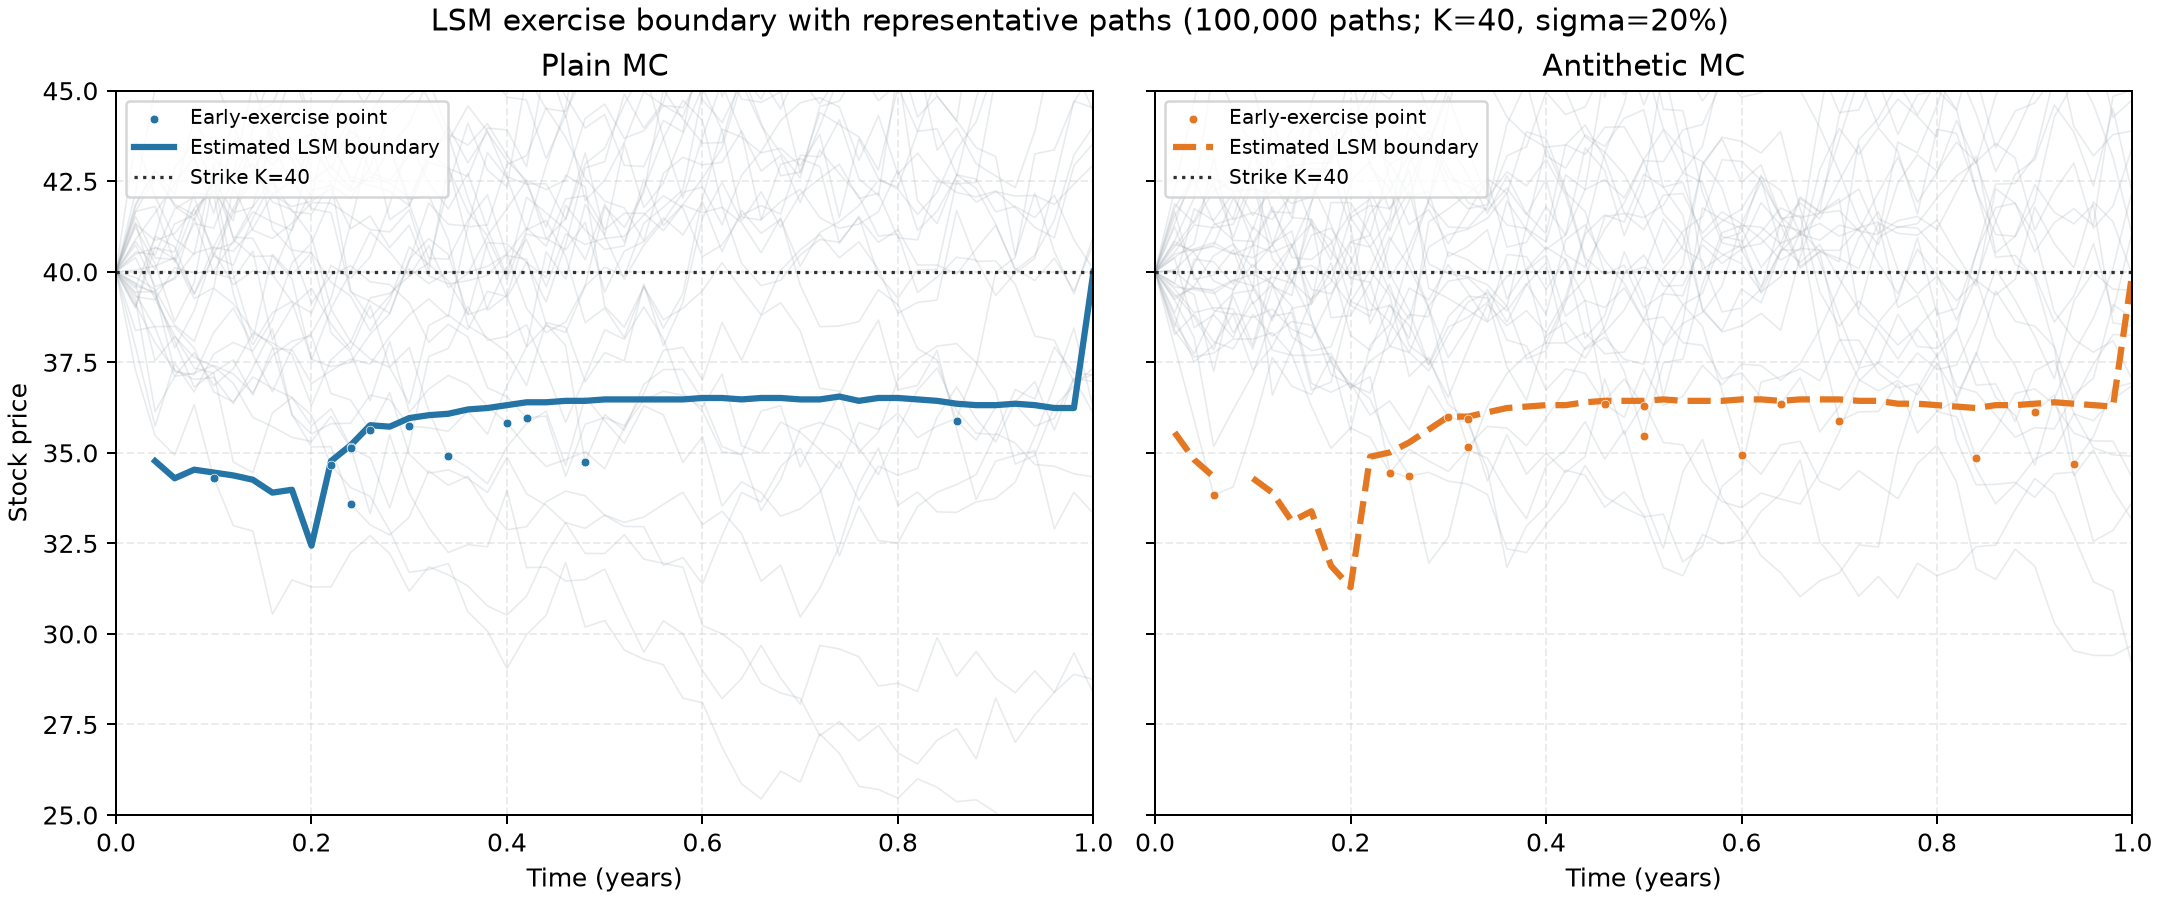
\includegraphics[width=\linewidth]{lsm_exercise_boundary.png}
    \caption{LSM fitted exercise boundary over representative simulated
    stock paths. Plain MC and AV panels use their respective native C++
    path samples; the bold curve is the estimated boundary and faint
    curves are sample paths.}
    \label{fig:lsm_exercise_boundary}
\end{figure}

The boundary is an illustrative grid estimate of the fitted stopping
rule, not an exact continuous-time boundary. Because the direct-state
basis produces an irregular boundary in this run, it should be read as a
diagnostic of this fitted policy rather than as an accurate economic
exercise boundary. Paths crossing into the exercise region illustrate the
rule; the plotted path subset is not used to define the boundary. All path simulation, regression, stopping
decisions, and CRR calculations are performed in the native C++ program;
Python is used only to assemble tables and create visualizations.
